Serieschaltung von Widerstand und Spule an einem Rechtecksignal $U_e$\\
\begin{tabular}{ccc} 
	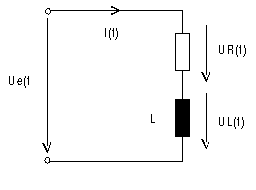
\includegraphics[width=3.5cm]{./idiotenseite/images/schaltung_spule.png} &
	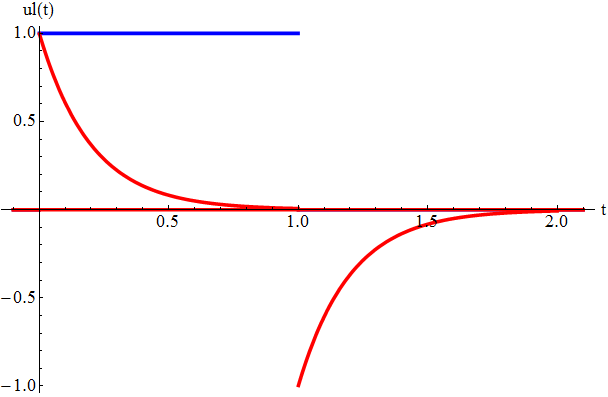
\includegraphics[width=3.5cm]{./idiotenseite/images/uSpule.png} &
	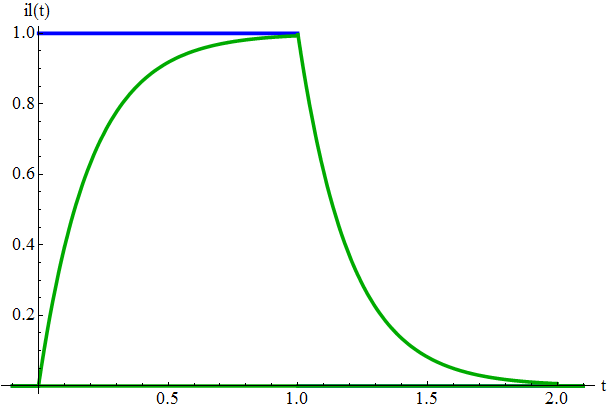
\includegraphics[width=3.5cm]{./idiotenseite/images/iSpule.png}\\	
\end{tabular}
\begin{multicols}{2}
	Ladevorgang\\
	$i_{\mathrm{L}} (t) = I_0 \cdot \biggl(1 - \mathrm{e}^{-
	\frac{t}{\tau}}\biggr) = \frac{U_0}{R_{\mathrm{L}}} \cdot \biggl(1 -
	\mathrm{e}^{- \frac{t \cdot R_{\mathrm{L}}}{L}}\biggr)$\\
	$u_{\mathrm{L}} (t) = \hat u \cdot e^{- \frac{t}{\tau}} = \hat u \cdot e^{-
	\frac{t \cdot R_{\mathrm{L}}}{L}}$\\
	\newline
	Entladevorgang\\
	$i_{\mathrm{L}} (t) = I_0 \cdot e^{- \frac{t}{\tau}} =
	\frac{U_0}{R_{\mathrm{L}}} \cdot e^{- \frac{t \cdot
	R_{\mathrm{L}}}{L}}$\\
	$u_{\mathrm{L}} (t) = - \hat u \cdot e^{- \frac{t}{\tau}} = - \hat u \cdot
	e^{- \frac{t \cdot R_{\mathrm{L}}}{L}}$\\
\end{multicols}

